\documentclass{standalone}
\usepackage{pgfplots}
\pgfplotsset{compat=1.18}
\usepgfplotslibrary{colorbrewer}
\pgfplotsset{cycle list/Set1-6}

\begin{document}

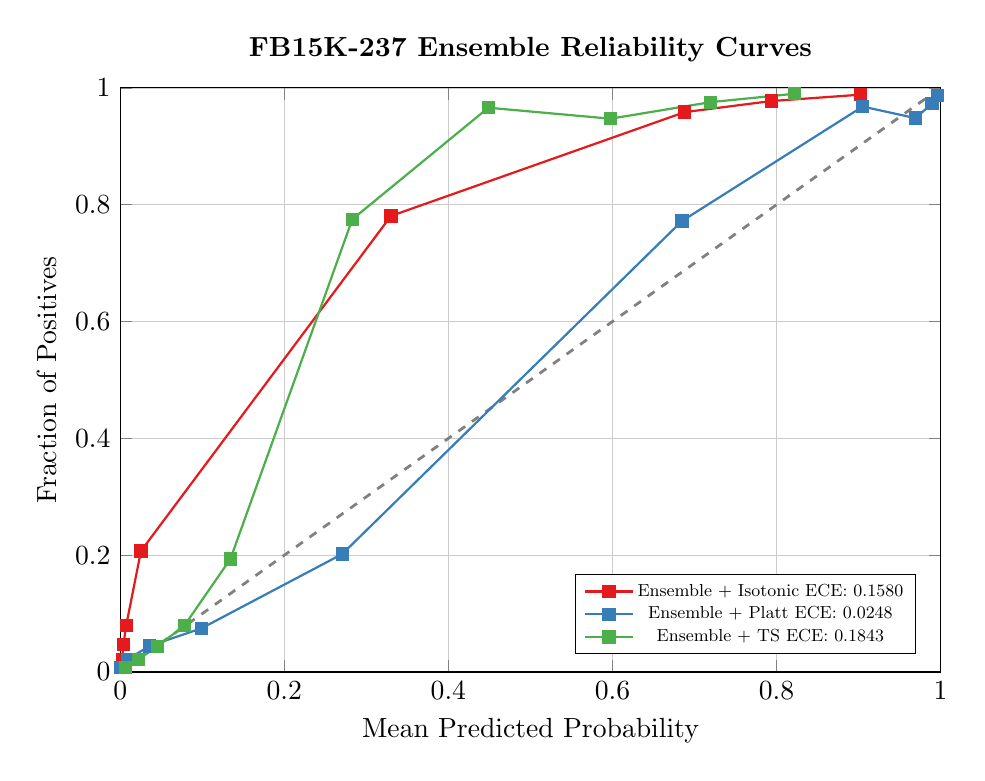
\begin{tikzpicture}
\begin{axis}[
    title={\textbf{FB15K-237 Ensemble Reliability Curves}},
    xlabel={Mean Predicted Probability},
    ylabel={Fraction of Positives},
    xmin=0, xmax=1,
    ymin=0, ymax=1,
    xtick={0, 0.2, 0.4, 0.6, 0.8, 1.0},
    ytick={0, 0.2, 0.4, 0.6, 0.8, 1.0},
    legend pos= south east,
    legend style={nodes={scale=0.7, transform shape}, font=\small},
    grid=both,
    grid style={line width=.1pt, draw=gray!20},
    major grid style={line width=.2pt, draw=gray!40},
    width=12cm,
    height=9cm,
    cycle list name=Set1-6
]

% Perfectly Calibrated Line
\addplot [color=gray, dashed, line width=1pt, forget plot]
    coordinates {(0,0)(1,1)};

\addplot+[mark=square*, thick] coordinates {
    (0.00240926, 0.00806058) (0.00244837, 0.02174444) (0.00386932, 0.04693354) 
    (0.00719773, 0.07961477) (0.02527953, 0.20719219) (0.32992911, 0.78064993) 
    (0.68794735, 0.95846060) (0.79345810, 0.97742770) (0.90225669, 0.98834197)
};
\addlegendentry{Ensemble + Isotonic ECE: 0.1580}


\addplot+[mark=square*, thick] coordinates {
    (0.00087264, 0.00830484) (0.00882599, 0.02150012) (0.03540569, 0.04446616) 
    (0.09900151, 0.07476179) (0.27066986, 0.20205228) (0.68469810, 0.77204984) 
    (0.90501012, 0.96799414) (0.96937633, 0.94820425) (0.98966927, 0.97336917) 
    (0.99654592, 0.98729849)
};
\addlegendentry{Ensemble + Platt ECE: 0.0248}

\addplot+[mark=square*, thick] coordinates {
    (0.00618313, 0.00781632) (0.02217479, 0.02150012) (0.04525506, 0.04397752) 
    (0.07813541, 0.07940386) (0.13429148, 0.19350110) (0.28287717, 0.77498168) 
    (0.44871354, 0.96603958) (0.59756261, 0.94722697) (0.71959271, 0.97556804) 
    (0.82231991, 0.98998534)
};
\addlegendentry{Ensemble + TS ECE: 0.1843}

\end{axis}
\end{tikzpicture}

\end{document}